%!TEX root=paper.tex


  \newpage
  \section{Service Utilization and Performance}

  % Since it is tailored for Flask applications, the deployment of \tool is trivial. 

  The tool is designed to take advantage of the fact that it runs in the same web application context and that the monitored API already has a web presence. It thus simply makes available one extra endpoint (i.e. \code{/dashboard}) at the same address as the API, endpoint which serves the interactive application presented in the remainder of this paper. 

  A dashboard can be attached to an already existing Flask application with a single line of code as the code in the following snippet shows
  \footnote{We do not count the import statement that enables that line}:

  % which binds the dashboard to a Flask application\footnote{\ins{ In this paper we present the integration with APIs written in Python and Flask hoping that this will not prevent the reader from seeing the more general idea; all the tools we show here for Flask can be applied to other API technologies (e.g. Django) by simply providing a few back-end adapters in the right places. }}:

  % caption=Configuring the \tool is straightforward,
  \begin{lstlisting}[style=custompython]
  import flask_monitoringdashboard as dashboard

  # LOC #1: associate the main Flask application 
  # object with the dashboard
  dashboard.bind(app) 

  \end{lstlisting}

  During binding, the \tool will search for all endpoints defined in the target application and make them available in the dashboard in an interactive configuration panel (\Fref{fig:sep}). The panel presents all the automatically discovered endpoints and lets the user select the ones that should be monitored (the checkboxes in the last column). When the user enables the monitoring of an endpoint a function wrapper is added to the implementation of that endpoint (which is a function in Flask). The information is also saved in a database such that it is persistent across application restarts. 

  

  % In order to monitor an endpoint, the \tool creates a function wrapper for the API function that corresponds to the endpoint. This way, the wrapper will be executed whenever that API call is made before the actual function is called. The wrapper contains the code that takes care of monitoring an endpoint. 

    \begin{figure}[h!]
      \centering
      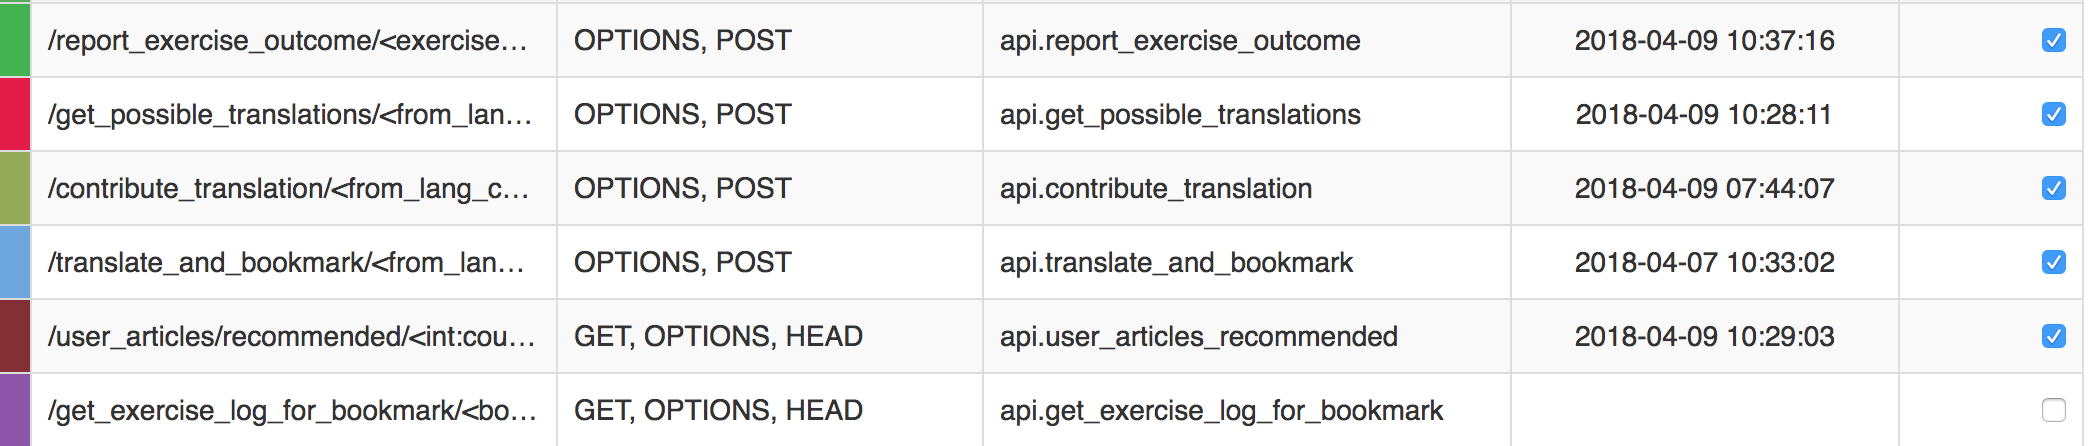
\includegraphics[width=\linewidth]{selecting_endpoints.png}
      \caption{Once connected to an API the Dashboard presents the endpoints that are available for monitoring}
      \label{fig:sep}
    \end{figure}

  By default the dashboard takes an {\em opt-in} approach to monitoring: to prevent the performance penalties incurred by the dashboard\footnote{We discuss performance issues later} to affect performance sensitive endpoints, the service developer is asked to manually add the endpoints they want to monitor. 
   

  One alternative to configuring the monitored endpoints from the user interface is to allow the service developer to annotate the code. This would however pollute the code, and prevent deploying two versions which would monitor different endpoints. Also, would pose problems with endpoint evolution in the future.

  
\niceseparator

  The remainder of this section presents several interactive
  visualizations that are available in the dashboared without any further configuration\footnote{We recommend obtaining a color version of this paper for better readability}. They are focused on two types of information that is important to the API maintainer: 

  \begin{itemize}

    \item {\bf Utilization} -- refers to how the third parties use the API, which parts are most used, which are little used, etc. This is known to be critical information for upstream developer in general\cite{Haen14a}. In the case of source code dependencies one can detect such information by analyzing software repositories. However, in the case of services, there is no other way but monitoring service utilization. 

    \item {\bf Performance} as measured in response times. This is important, especially for APIs that are supposed to be integrated in live systems. 

  \end{itemize}
